%%%%%%%%%%%%%%%%%%%%%%%%%%%%%%%%%%%%%%%%%
% Beamer Presentation
% LaTeX Template
% Version 1.0 (10/11/12)
%
% This template has been downloaded from:
% http://www.LaTeXTemplates.com
%
% License:
% CC BY-NC-SA 3.0 (http://creativecommons.org/licenses/by-nc-sa/3.0/)
%
%%%%%%%%%%%%%%%%%%%%%%%%%%%%%%%%%%%%%%%%%

%----------------------------------------------------------------------------------------
%	PACKAGES AND THEMES
%----------------------------------------------------------------------------------------

\documentclass{beamer}

\mode<presentation> {

% The Beamer class comes with a number of default slide themes
% which change the colors and layouts of slides. Below this is a list
% of all the themes, uncomment each in turn to see what they look like.

%\usetheme{default}
%\usetheme{AnnArbor}
%\usetheme{Antibes}
%\usetheme{Bergen}
%\usetheme{Berkeley}
%\usetheme{Berlin}
%\usetheme{Boadilla}
%\usetheme{CambridgeUS}
%\usetheme{Copenhagen}
%\usetheme{Darmstadt}
%\usetheme{Dresden}
%\usetheme{Frankfurt}
%\usetheme{Goettingen}
%\usetheme{Hannover}
%\usetheme{Ilmenau}
%\usetheme{JuanLesPins}
%\usetheme{Luebeck}
\usetheme{Madrid}
%\usetheme{Malmoe}
%\usetheme{Marburg}
%\usetheme{Montpellier}
%\usetheme{PaloAlto}
%\usetheme{Pittsburgh}
%\usetheme{Rochester}
%\usetheme{Singapore}
%\usetheme{Szeged}
%\usetheme{Warsaw}

% As well as themes, the Beamer class has a number of color themes
% for any slide theme. Uncomment each of these in turn to see how it
% changes the colors of your current slide theme.

%\usecolortheme{albatross}
%\usecolortheme{beaver}
%\usecolortheme{beetle}
%\usecolortheme{crane}
%\usecolortheme{dolphin}
%\usecolortheme{dove}
%\usecolortheme{fly}
%\usecolortheme{lily}
%\usecolortheme{orchid}
%\usecolortheme{rose}
%\usecolortheme{seagull}
%\usecolortheme{seahorse}
%\usecolortheme{whale}
%\usecolortheme{wolverine}

%\setbeamertemplate{footline} % To remove the footer line in all slides uncomment this line
%\setbeamertemplate{footline}[page number] % To replace the footer line in all slides with a simple slide count uncomment this line

%\setbeamertemplate{navigation symbols}{} % To remove the navigation symbols from the bottom of all slides uncomment this line
}

\usepackage{graphicx} % Allows including images
\usepackage{booktabs} % Allows the use of \toprule, \midrule and \bottomrule in tables
\usepackage{movie15}
\usepackage{textcomp}
\usepackage{hyperref}
\hypersetup{
    colorlinks=true,
    linkcolor=blue,
    filecolor=magenta,      
    urlcolor=blue,
}
\urlstyle{same}

%\usepackage{quotchap}
%----------------------------------------------------------------------------------------
%	TITLE PAGE
%----------------------------------------------------------------------------------------

\title[Short title]{Deep Reinforcement Learning for control, investigating the application to a trajectory planning problem } % The short title appears at the bottom of every slide, the full title is only on the title page

\author{Lars Klein} % Your name
\institute[PEM] % Your institution as it will appear on the bottom of every slide, may be shorthand to save space
{
RWTH \\ % Your institution for the title page
\medskip
\textit{lars.klein@rwth-aachen.de} % Your email address
}
\date{\today} % Date, can be changed to a custom date

\begin{document}

\begin{frame}
\titlepage % Print the title page as the first slide
\end{frame}

\begin{frame}
\frametitle{Overview} % Table of contents slide, comment this block out to remove it
\tableofcontents % Throughout your presentation, if you choose to use \section{} and \subsection{} commands, these will automatically be printed on this slide as an overview of your presentation
\end{frame}

%----------------------------------------------------------------------------------------
%	PRESENTATION SLIDES
%----------------------------------------------------------------------------------------

%------------------------------------------------
\section{Orientation}
\subsection{What is RL}
\subsection{What is the scope of this presentation}

\begin{frame}
\frametitle{Orientation (Disorientation ? )}
\begin{figure}
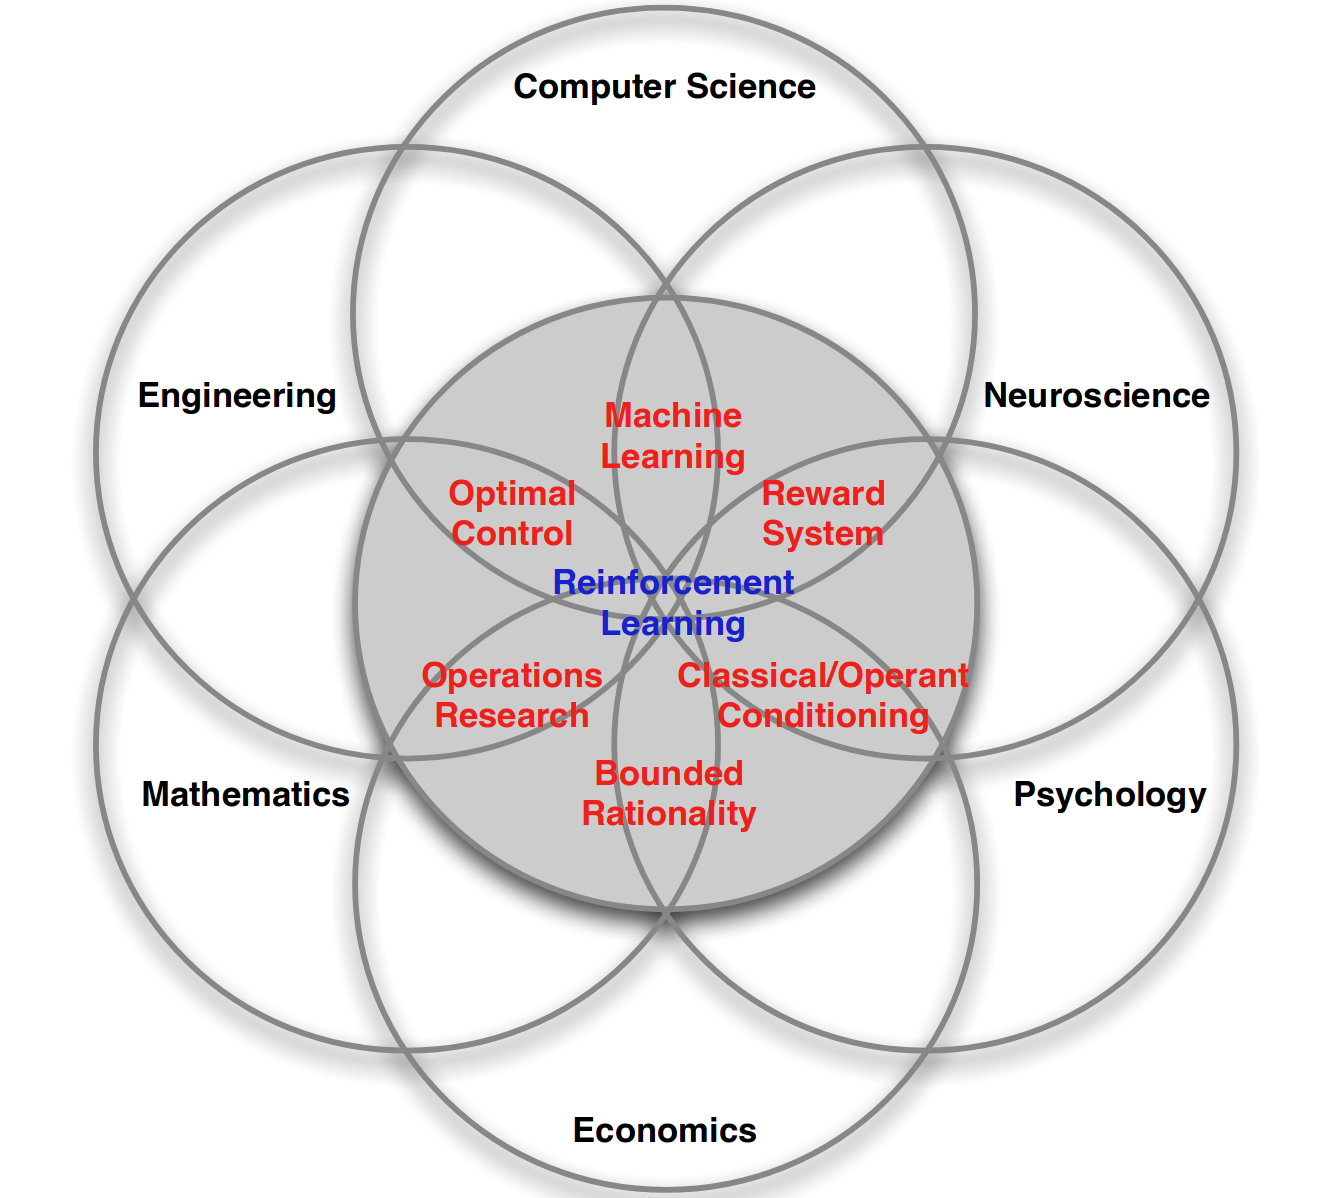
\includegraphics[height=0.7\textheight]{venn_rl}
\end{figure}
\end{frame}

%------------------------------------------------

\begin{frame}
\frametitle{What is the scope of this presentation?}
Reinforcement learning can be presented from many perspectives.
An exhaustive discussion is beyond the scope of this presentation.
Instead we will focus on
\begin{itemize}
\item A short intro to machine learning
\item Description of a reinforcement learning problem
\item Introduction to one of the key algorithms
\item Demo of my simulation
\item Discussion of results and problems
\end{itemize}
\end{frame}

\begin{frame}
\frametitle{Intro to Machine Learning}
\begin{figure}
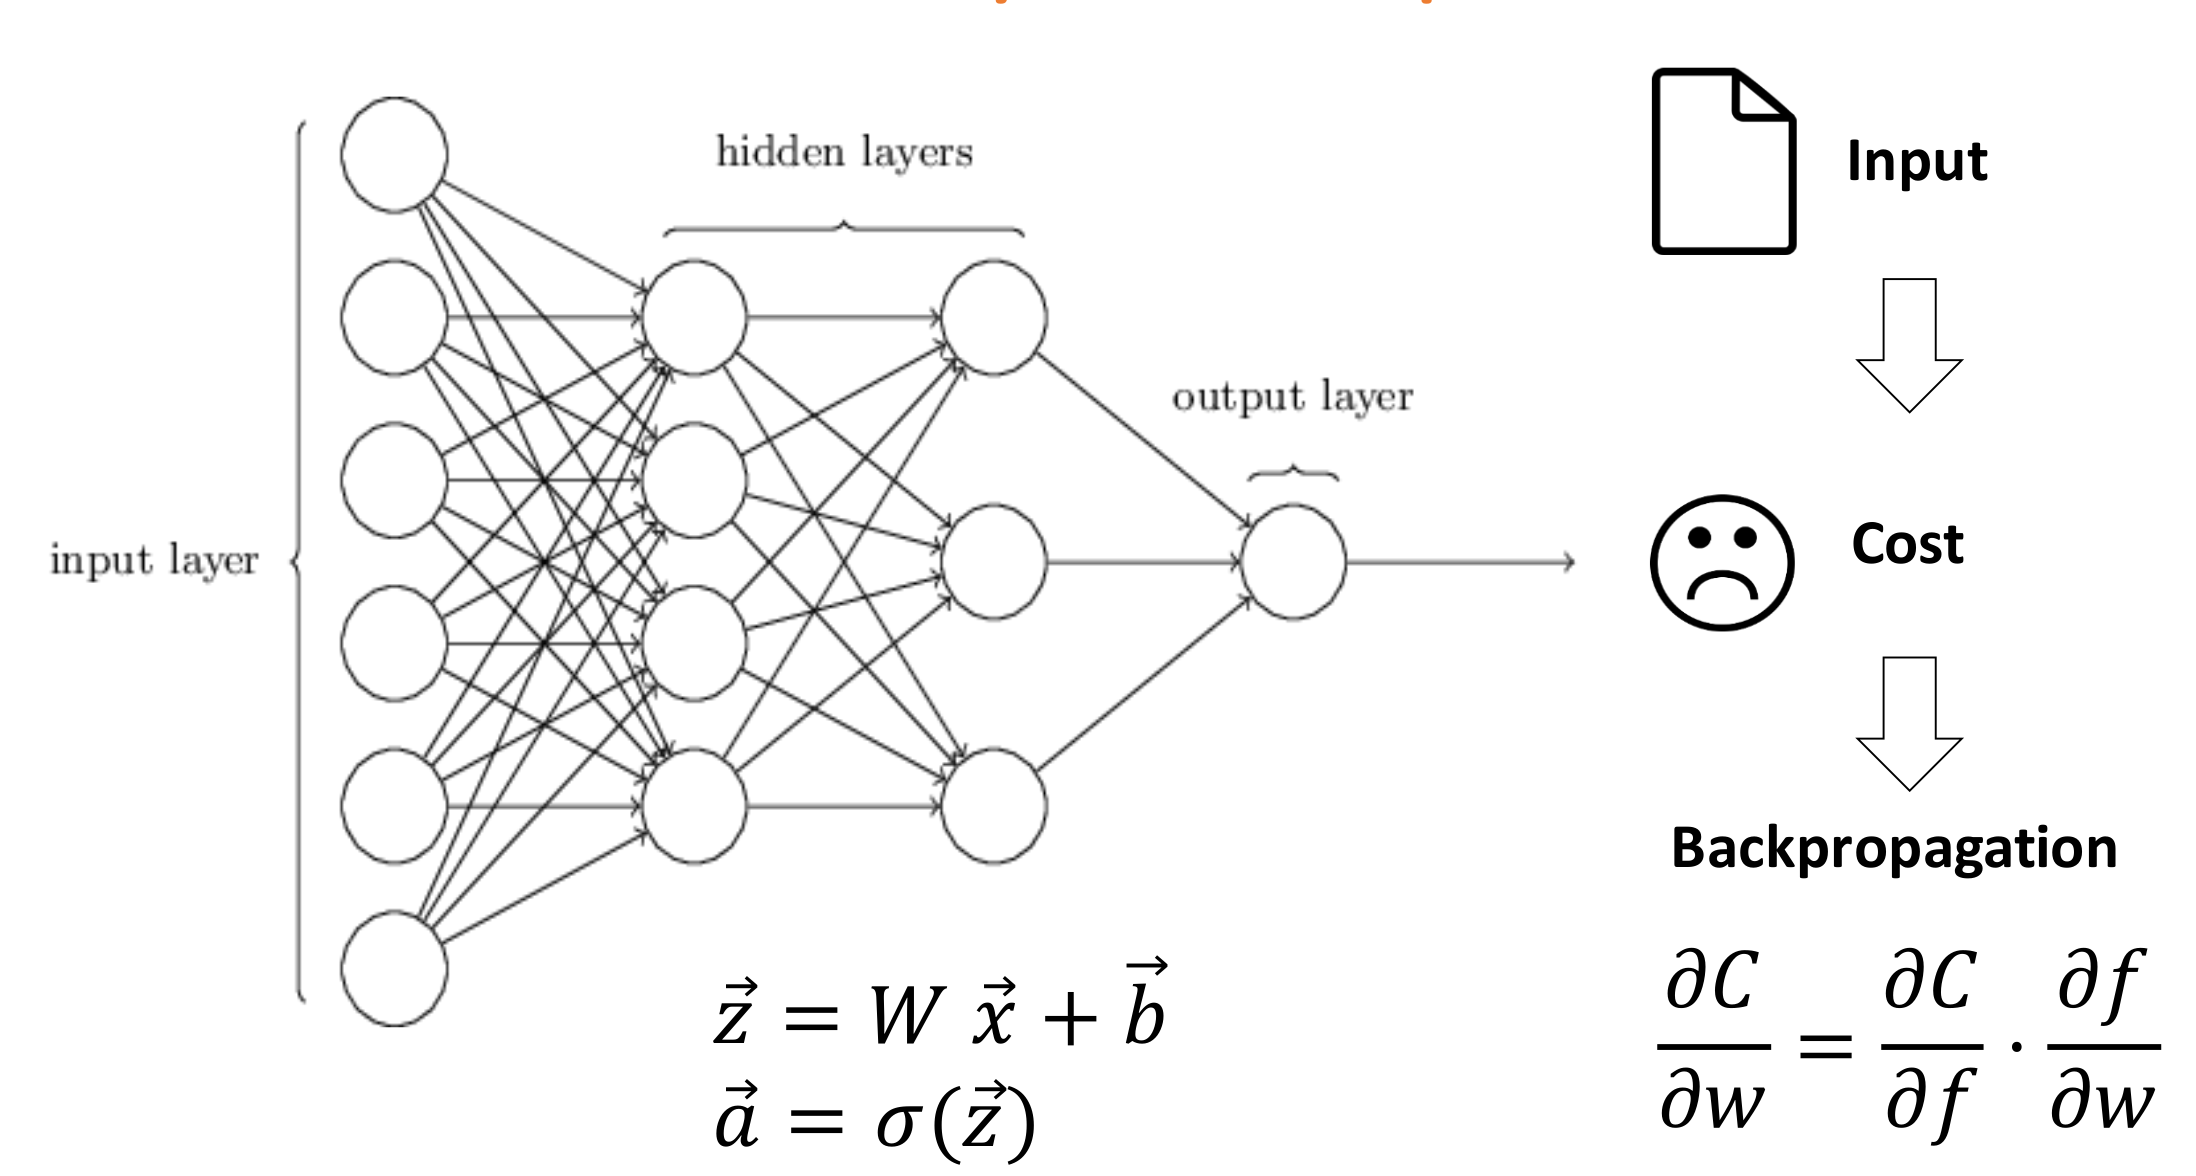
\includegraphics[height=0.7\textheight]{ml_slide.png}
\end{figure}
\end{frame}

%------------------------------------------------

\begin{frame}
\frametitle{Types of Machine Learning}
\begin{block}{Unsupervised}
You are given only data. The goal is to find structure within this data. Typical tasks would be compression or outlier detection.
\end{block}

\begin{block}{Supervised}
You are given pairs of  \((input, output)\). The goal is to learn a good prediction of outputs for new inputs.
This is further divided into \textbf{Regression} \(predicting continuous outputs\) and \textbf{Classification} \(predicting discrete outputs\).
\end{block}

\begin{block}{Reinforcement learning}
You are given a simulation that you can interact with, and a feedback signal that informs you how well you did. The goal is to explore behaviours and identify a strategy to maximize positive feedback.
\end{block}
\end{frame}

%------------------------------------------------
\begin{frame}
\frametitle{Challenges in reinforcement learning}
The purpose of reinforcement learning is to predict values for behaviours.
But this is not just regression for reward signals:
\begin{itemize}
\item Data is created interactively.
\item Reward can be sparse
\item Reward can be delayed
\item Reward can be non-deterministic
\item State of the simulation can be very complex
\item State of the simulation can be only partially observable
\end{itemize}
\bigskip

The reinforcement agent needs to discover viable strategies while exploring the simulation.\\
\textrightarrow  Simulation needs to be designed in tandem with the rl algorithm.
\end{frame}

\begin{frame}
\frametitle{A typical RL agent}
\begin{figure}
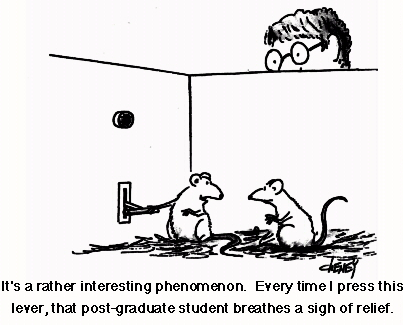
\includegraphics[width=0.8\textwidth]{rat_cartoon.jpg}
\end{figure}
\end{frame}

\begin{frame}
\begin{center}
\textbf{So how does it actually look ?}
\end{center}
\end{frame}

\begin{frame}
\frametitle{Definitions}
An interaction with the environment: \(S_t, a_t, r_t \rightarrow S_{t+1}\) :
\begin{itemize}
\item \(s_t \in S\) state (partial observation) at time t
\item \(a_t \in A\) action taken at time t
\item \(r_t\) reward received at time t
\item \(s_{t+1}\) state (partial observation) at time t+1
\item \(a_t \sim \pi(s_t) = P(a \in A | s_t \in S)\), actions are drawn from a distribution over the action space A, conditioned on the current state.
\end{itemize}
\bigskip
The reward \(r_t\) obtained at time t, as well as the next state \(s_{t+1}\) depend on the action \(a_t\) sampled from \(\pi\).
\end{frame}

\begin{frame}
\frametitle{Definitions}
All interactions with the environment are based on a policy. We derive the following definitions:
\begin{itemize}
\item \(v(s) = E_{\pi, s_t = s}(r_t) + \mu * E_{\pi, s_t = s}(v(s_{t+1})\), the \textbf{value} of a state.\\
Defined as total expected future reward.\\
A discount factor \(\mu\) is introduced to avoid infinite values.\\
The recursion stops at terminal states with a fixed value of 0.
\item \(Q(s, a) = E_{\pi, s_t = s, a_t= a} (v(s))\), analogous to value, \\
but action at time t is already given
\item \(A(s, a) = Q(s, a) - v(s)\), advantage of choosing action a at state s.
\end{itemize}
\end{frame}

\begin{frame}
\frametitle{How to act ?}
The goal is to maximize the total expected future reward:
\begin{itemize}
\item \(\pi^\star\) is the ideal policy. \\
\hspace{0.5cm} \textrightarrow  \hspace{0.5cm} \(a_t \sim \pi^\star(s_t)\). 
\item \(Q^\star(a, s)\) are the Q-values associated with the ideal policy.\\
\hspace{0.5cm} \textrightarrow  \hspace{0.5cm} \(a_t = argmax_a Q^\star(s_t, a)\)
\item \(A^\star(a, s)\) are the advantages associated with the ideal policy. \\
Please note: \(A^\star <= 0\)
\end{itemize}
\bigskip

For continous action spaces:
\begin{itemize}
\item \(\pi\) is a probability distribution, it translates nicely to the sampling of continous instead of discrete actions.
\item acting according to the Q values becomes problematic: Q can be very non-smooth and the evaluation is expensive.\\
\hspace{0.5cm} \textrightarrow  \hspace{0.5cm} the argmax becomes a complex optimization problem.
\end{itemize}
\end{frame}

\begin{frame}
\frametitle{Learning with policy gradients}
Policy gradient methods predict:
\begin{itemize}
\item policy \(\pi(s)\)
\item value \(v(s)\)
\end{itemize}
The value function is necessary for training the agent. \\
We use it to calculate an estimation of the advantage. \\
All notation here assumes empirical observations of rewards and states:
\begin{align*}
\delta_t &= -v(s_t) + r_t + \gamma  v(s_{t+1}) \\
\hat{A}(s_0 &=s, a_0 =0) = \sum_{t=0}^{\inf} \delta_t (\mu \gamma) ^t
\end{align*}
If we collect enough such estimates, we can approximate the true advantage function (which was defined as an expectation).\\
\textbf{Please note}: we assume a given initial action.
\end{frame}

\begin{frame}
\frametitle{Learning with policy gradients part 2}
Positive advantage = action is better than current policy,\\
negative advantage = action is worse\\
\hspace{0.5cm} \textrightarrow  \hspace{0.5cm} change the probability according to our advantage estimation.\\
\bigskip
In a machine learning setup:
\begin{itemize}
    \item updates become training steps
    \item \(\pi(s) = \pi_\theta(s)\), \\
        function approximator with parameters \(\theta\).
    \item estimate training gradients on empirical data:
\end{itemize}
\bigskip
\begin{large}
\[\hat{g}= \hat{E}(\nabla_\theta (log(\pi_\theta(a_0, s_0)) \: \hat{A}(a_0, s_0)\]
\end{large}
\end{frame}

\begin{frame}
\frametitle{Learning with policy gradients part 3}
In practice this leads to the following setup:
\begin{enumerate}
\item initialize random policy and random value prediction
\item interact with simulation and collect (lots of) observations
\item use observations to calculate empirical estimates,\\
      (advantages for each action)
\item train on empirical estimates \textrightarrow \hspace{0.2cm} update policy and value estimates
\item back to step 2.
\end{enumerate}
\end{frame}


\begin{frame}
\frametitle{Learning with policy gradients part 4}
Basically, we are repeating two steps:
\begin{itemize}
    \item use $\pi$ to get the value function $ v = v^\pi$
    \item update the policy with the value function $\pi := greedy(v)$
\end{itemize}
\bigskip
This is supposed to guarantee convergence. \\
At least that's what they say \href{http://www0.cs.ucl.ac.uk/staff/d.silver/web/Teaching_files/DP.pdf}{here}.\\
\bigskip
In practice, things look different ...
\end{frame}

\begin{frame}
\frametitle{Demo}
\begin{center}
A concrete RL task.
\end{center}
\end{frame}

\begin{frame}
\frametitle{Using OpenAI baseline algorithms}
\begin{center}
Two different reward setups:
\end{center}
\begin{figure}
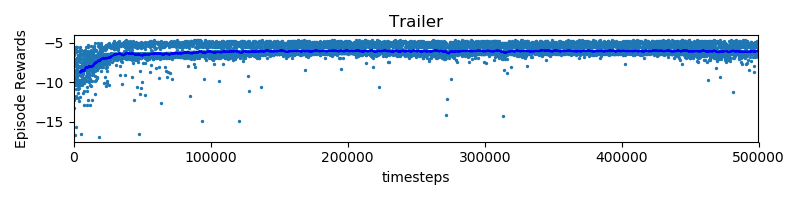
\includegraphics[width=0.95\textwidth]{zero_rew.png}\\
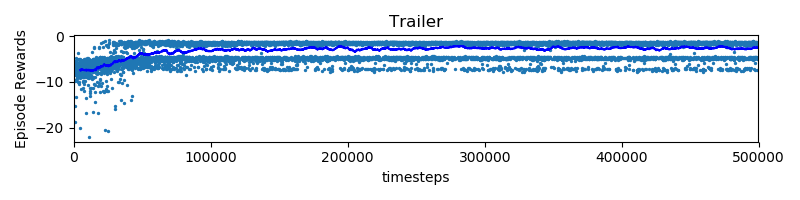
\includegraphics[width=0.95\textwidth]{pos_rew.png}
\end{figure}
\end{frame}

\begin{frame}
\frametitle{Tuning}
After reimplementing the algorithm and searching for better function approximators:\\
\begin{center}
\includemovie{5cm}{5cm}{agent.gif}
\end{center}
\end{frame}


%------------------------------------------------

\begin{frame}
\Huge{\centerline{Questions ?}}
\vspace{\fill}
\begin{footnotesize}
    Sources for the graphics (click me):
    \begin{itemize}
        \item \href{http://www.sharelatex.com}{venn diagram on reinforcement learning}
        \item \href{http://www2.smumn.edu/facpages/~dbucknam/}{rat comic}
        \item the others are homemade
    \end{itemize}
\end{footnotesize}

\end{frame}

%----------------------------------------------------------------------------------------

\end{document}